% Report 6 contribution: Nguyen Lu Nhat Huy (CE181196).
% Match the common Report6 preamble; no additional packages required.
\subsection{Public Profiles, Account Settings and Client Workspace}

\subsubsection{M1.07 -- View Public Client Profile}
\begin{itemize}[leftmargin=1.5em,itemsep=2pt]
  \item \textbf{Screen Name \& Route Path:}\newline \texttt{/clients/[id]}; Find Clients profile panel.
  \item \textbf{Target Actor:} Guest or authenticated user.
  \item \textbf{Preconditions:} The URL contains an existing Client user ID.
  \item \textbf{Purpose:} Read the published Client and company information.
\end{itemize}
\paragraph{Screen-Transition Workflow:} Find Work $\rightarrow$ Find Clients $\rightarrow$ View profile $\rightarrow$ Client profile panel $\rightarrow$ close to return.
\begin{figure}[H]\centering
\scalebox{0.61235}{%
\begingroup\setlength{\unitlength}{1pt}\linethickness{0.9pt}
\begin{picture}(450.00,253.12)
\put(0,0){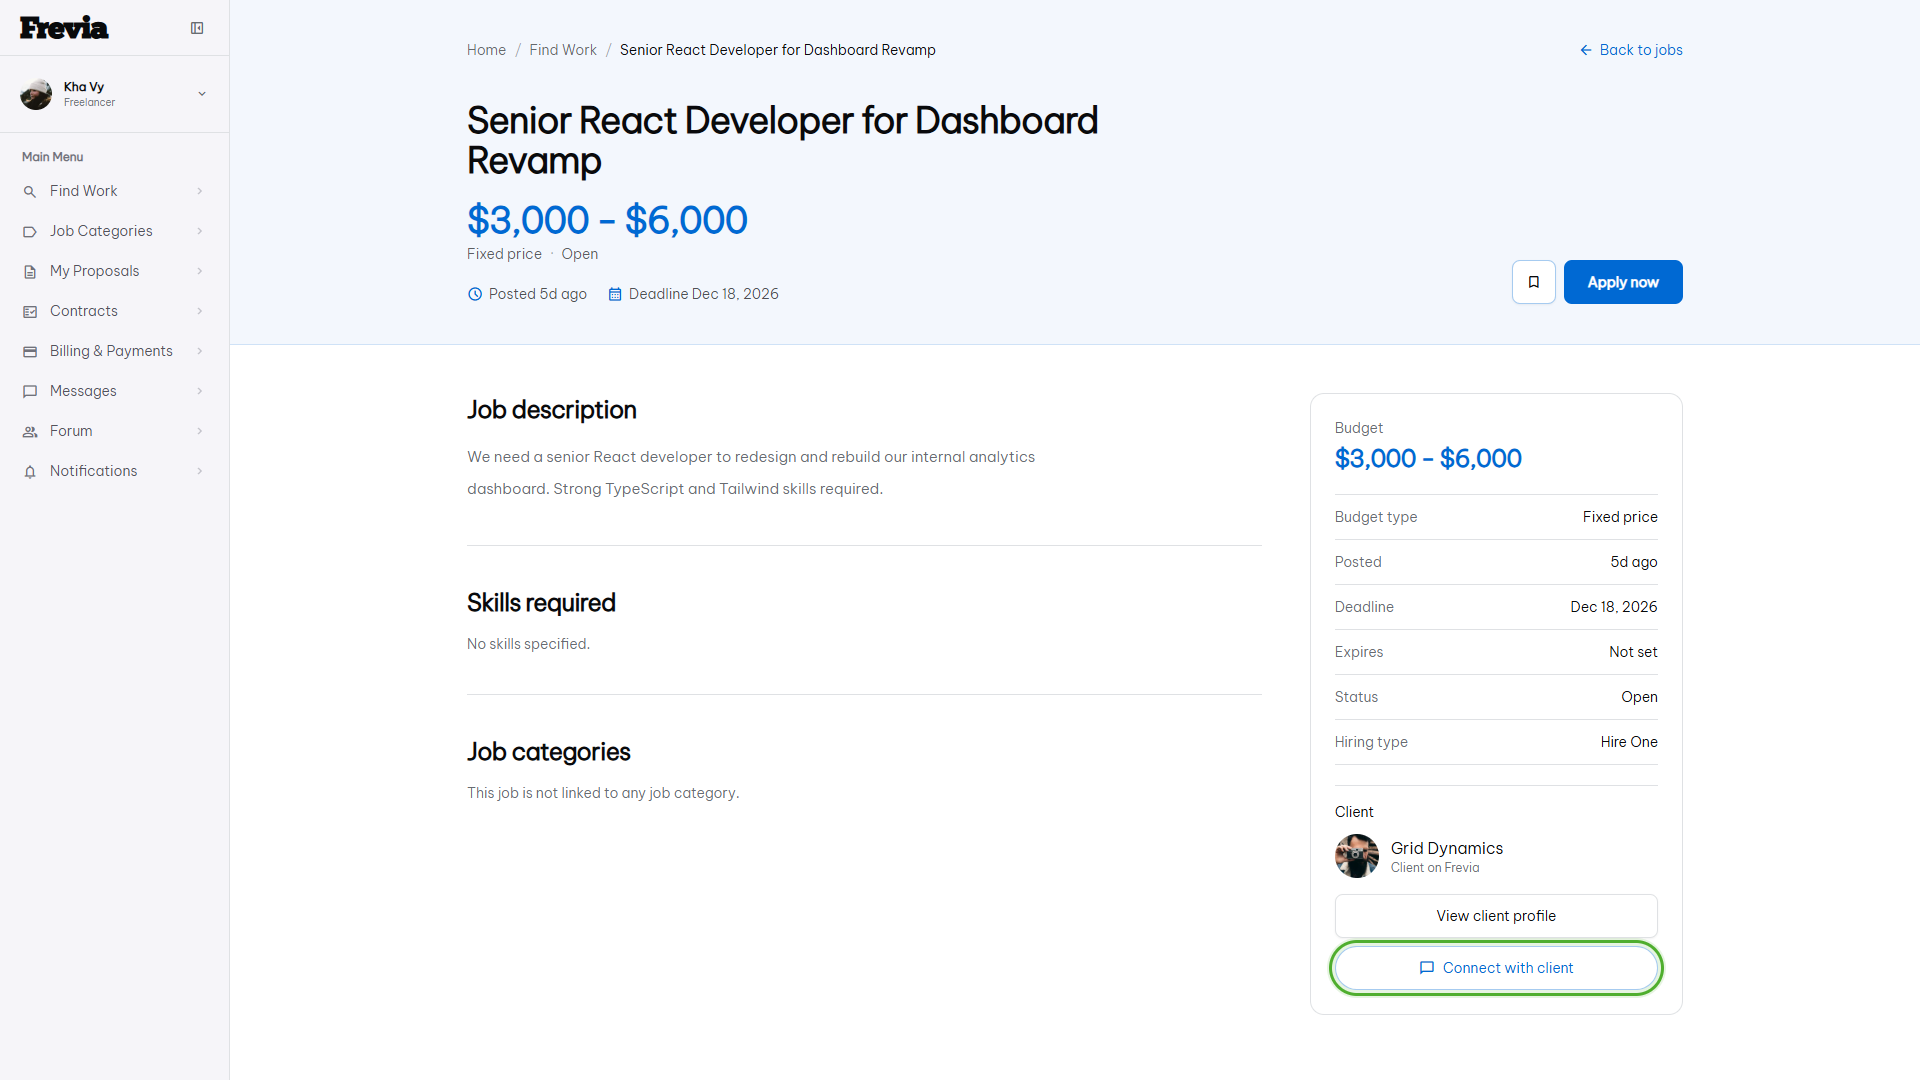
\includegraphics[width=450.00pt]{images/client/m1_07_view_client_profile_entry.png}}
\put(312.30,32.91){\color{fptred}\framebox(76.95,11.39){}}
\put(312.30,44.30){\colorbox{white}{\textcolor{fptred}{\scriptsize\bfseries 1}}}
\end{picture}
\endgroup}%
\caption{View client profile entry on a job detail page.}
\label{fig:r6_m1_07_view_client_profile_entry}
\end{figure}
\paragraph{Step-by-Step User Instructions:}
\begin{enumerate}[leftmargin=1.8em,itemsep=3pt]
  \item \rbadge{1} Open Find Work, select Find Clients and search for a Client. Select View profile. Alternatively, use View client profile on a job detail page.
  \item \rbadge{2} Read Client contact, the biography, company information and Social links in the Client profile panel. A missing website is shown as Website not provided; open a website only when a link is available.
  \item \rbadge{3} Close the panel using the top-right icon to return to Find Clients. Visitors cannot edit another Client's profile.
\end{enumerate}
\paragraph{Expected Output \& Exception Handling:}
\begin{itemize}[leftmargin=1.5em,itemsep=2pt]
  \item \textbf{Expected result:} The published Client profile is displayed; an unapproved draft is not treated as published data.
  \item \textbf{Troubleshooting:} If loading fails, use the retry control. Verify the ID and the API connection; an unavailable profile cannot be edited by a visitor.
\end{itemize}

\newpage
\subsubsection{M1.08 -- Public Expert Directory -- Availability}
\begin{itemize}[leftmargin=1.5em,itemsep=2pt]
  \item \textbf{Screen Name \& Route Path:}\newline \texttt{/experts (not available in this checkout)}.
  \item \textbf{Target Actor:} Guest or authenticated user.
  \item \textbf{Preconditions:} None for this release-status check.
  \item \textbf{Purpose:} Clarify the availability of the Expert directory listed in the checklist.
\end{itemize}
\guide{Release note: No public Expert directory page exists under the current web application routes. No working directory, search, or public Expert detail page is claimed here.}
\paragraph{Screen-Transition Workflow:} Checklist directory item $\rightarrow$ release availability check.
\paragraph{Step-by-Step User Instructions:}
\begin{enumerate}[leftmargin=1.8em,itemsep=3pt]
  \item \rbadge{1} Do not use \texttt{/experts} as a supported public navigation destination in this version.
  \item \rbadge{2} Use the dispute workflow when an assigned Expert is required. Expert operations currently use the permission-controlled Admin Portal.
\end{enumerate}
\paragraph{Expected Output \& Exception Handling:}
\begin{itemize}[leftmargin=1.5em,itemsep=2pt]
  \item \textbf{Expected result:} The guide does not direct users to a missing screen.
  \item \textbf{Troubleshooting:} A missing route is a release gap, not a permission that a Client should grant to themselves.
\end{itemize}

\newpage
\subsubsection{M3.01 -- Update Personal Information}
\begin{itemize}[leftmargin=1.5em,itemsep=2pt]
  \item \textbf{Screen Name \& Route Path:}\newline \texttt{/freelancer/profile or /client/profile}.
  \item \textbf{Target Actor:} Freelancer or Client.
  \item \textbf{Preconditions:} Signed in with the corresponding active role.
  \item \textbf{Purpose:} Maintain account display name and biography.
\end{itemize}
\guide{Release note: This form exposes display name and bio. Phone, address and timezone fields must not be inferred from the checklist. The latest local overview opens an editor rather than making every displayed value directly editable.}
\paragraph{Screen-Transition Workflow:} Profile settings $\rightarrow$ Personal information $\rightarrow$ Edit personal information $\rightarrow$ save or submit for review.
\begin{figure}[H]\centering
\scalebox{0.9288}{%
\begingroup\setlength{\unitlength}{1pt}\linethickness{0.9pt}
\begin{picture}(450.00,226.09)
\put(0,0){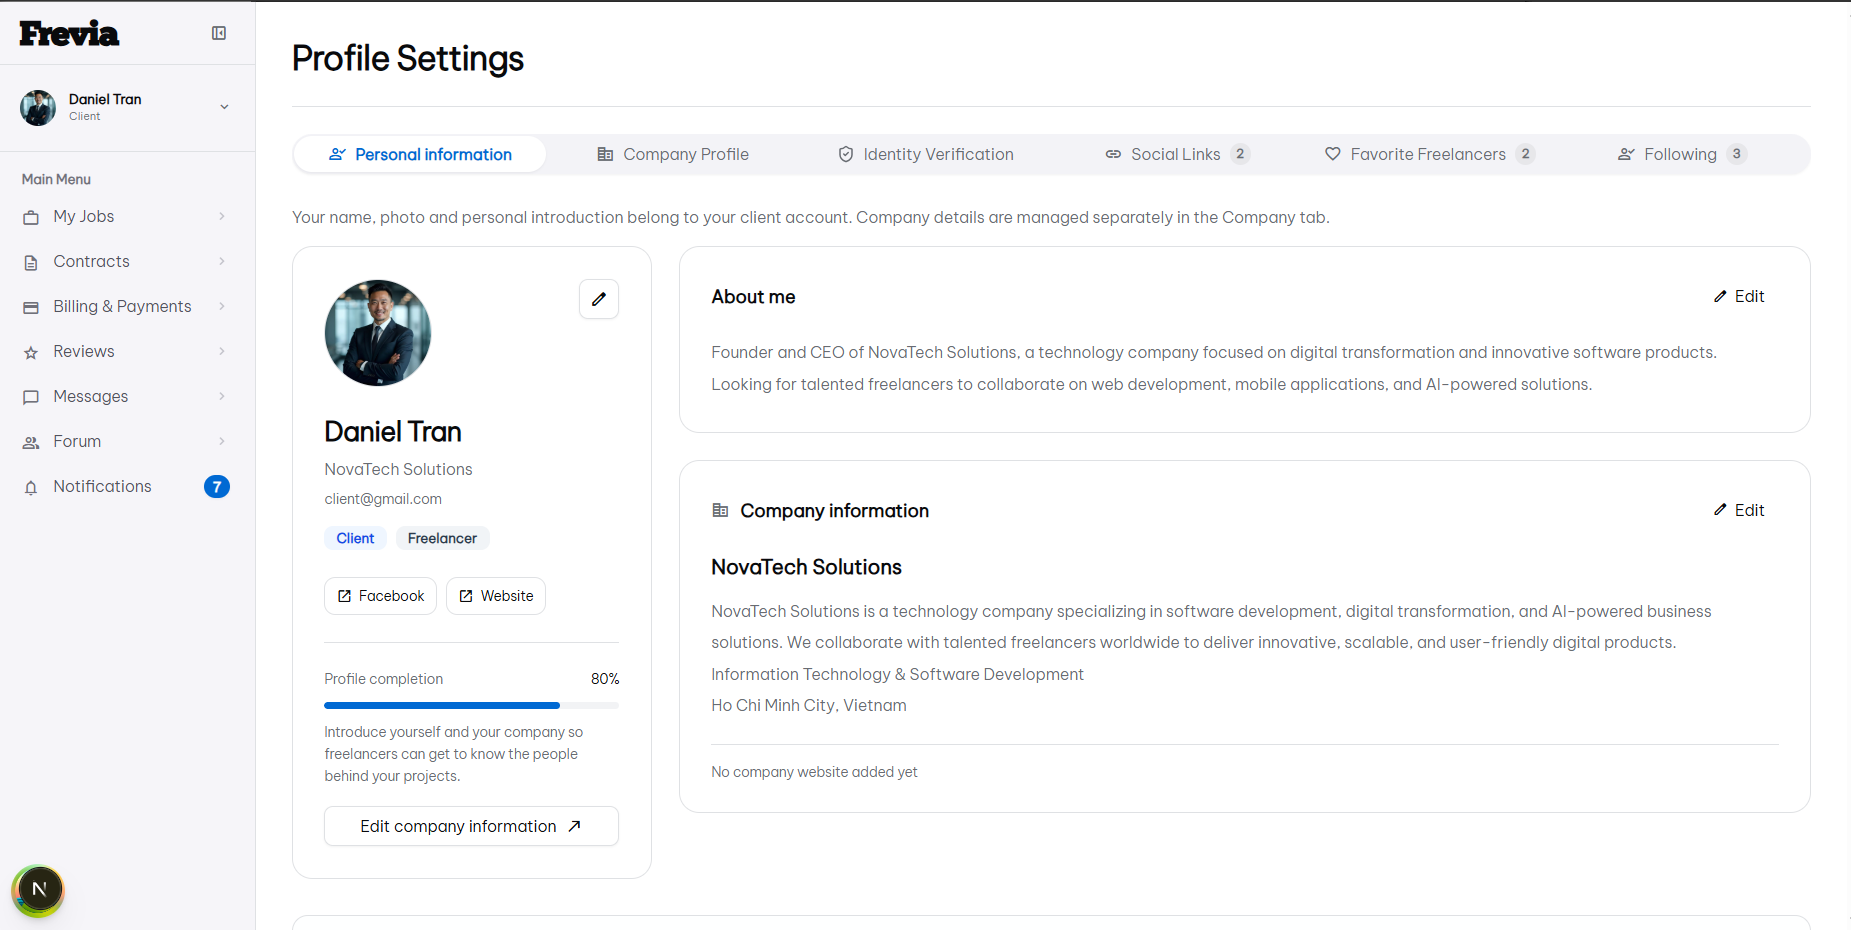
\includegraphics[width=450.00pt]{images/client/m3_01_view_client_profile.png}}
\put(414.90,147.41){\color{fptred}\framebox(20.25,12.43){}}
\put(414.90,159.85){\colorbox{white}{\textcolor{fptred}{\scriptsize\bfseries 1}}}
\end{picture}
\endgroup}%

\caption{Client Personal information overview; edit actions are on the right.}
\label{fig:r6_m3_01_view_client_profile}
\end{figure}
\paragraph{Step-by-Step User Instructions:}
\begin{enumerate}[leftmargin=1.8em,itemsep=3pt]
  \item \rbadge{1} Open your profile settings and select Personal information.
  \item \rbadge{2} Choose the personal-information edit action. Update Display name and Bio; leave the email unchanged because it is not edited through this form.
  \item \rbadge{3} Save the form once. Read the result and any pending-review notice before closing the editor.
\end{enumerate}
\paragraph{Expected Output \& Exception Handling:}
\begin{itemize}[leftmargin=1.5em,itemsep=2pt]
  \item \textbf{Expected result:} A successful save updates the permitted account information or records a pending profile revision according to the review policy.
  \item \textbf{Troubleshooting:} Correct field validation errors in the editor. A pending revision does not mean that every proposed value has already replaced the public profile.
\end{itemize}

\newpage
\subsubsection{M3.02 -- Upload Profile Photo}
\begin{itemize}[leftmargin=1.5em,itemsep=2pt]
  \item \textbf{Screen Name \& Route Path:}\newline \texttt{/freelancer/profile or /client/profile}.
  \item \textbf{Target Actor:} Freelancer or Client.
  \item \textbf{Preconditions:} Signed in; an image file is available.
  \item \textbf{Purpose:} Replace the account avatar.
\end{itemize}
\guide{Release note: There is no crop tool in the inspected upload form. Crop the image before selecting it if needed; this guide does not invent an in-app crop step.}
\paragraph{Screen-Transition Workflow:} Personal information $\rightarrow$ photo editor $\rightarrow$ choose image $\rightarrow$ Upload photo.
\begin{figure}[H]\centering
\scalebox{0.93665}{%
\begingroup\setlength{\unitlength}{1pt}\linethickness{0.9pt}
\begin{picture}(450.00,218.10)
\put(0,0){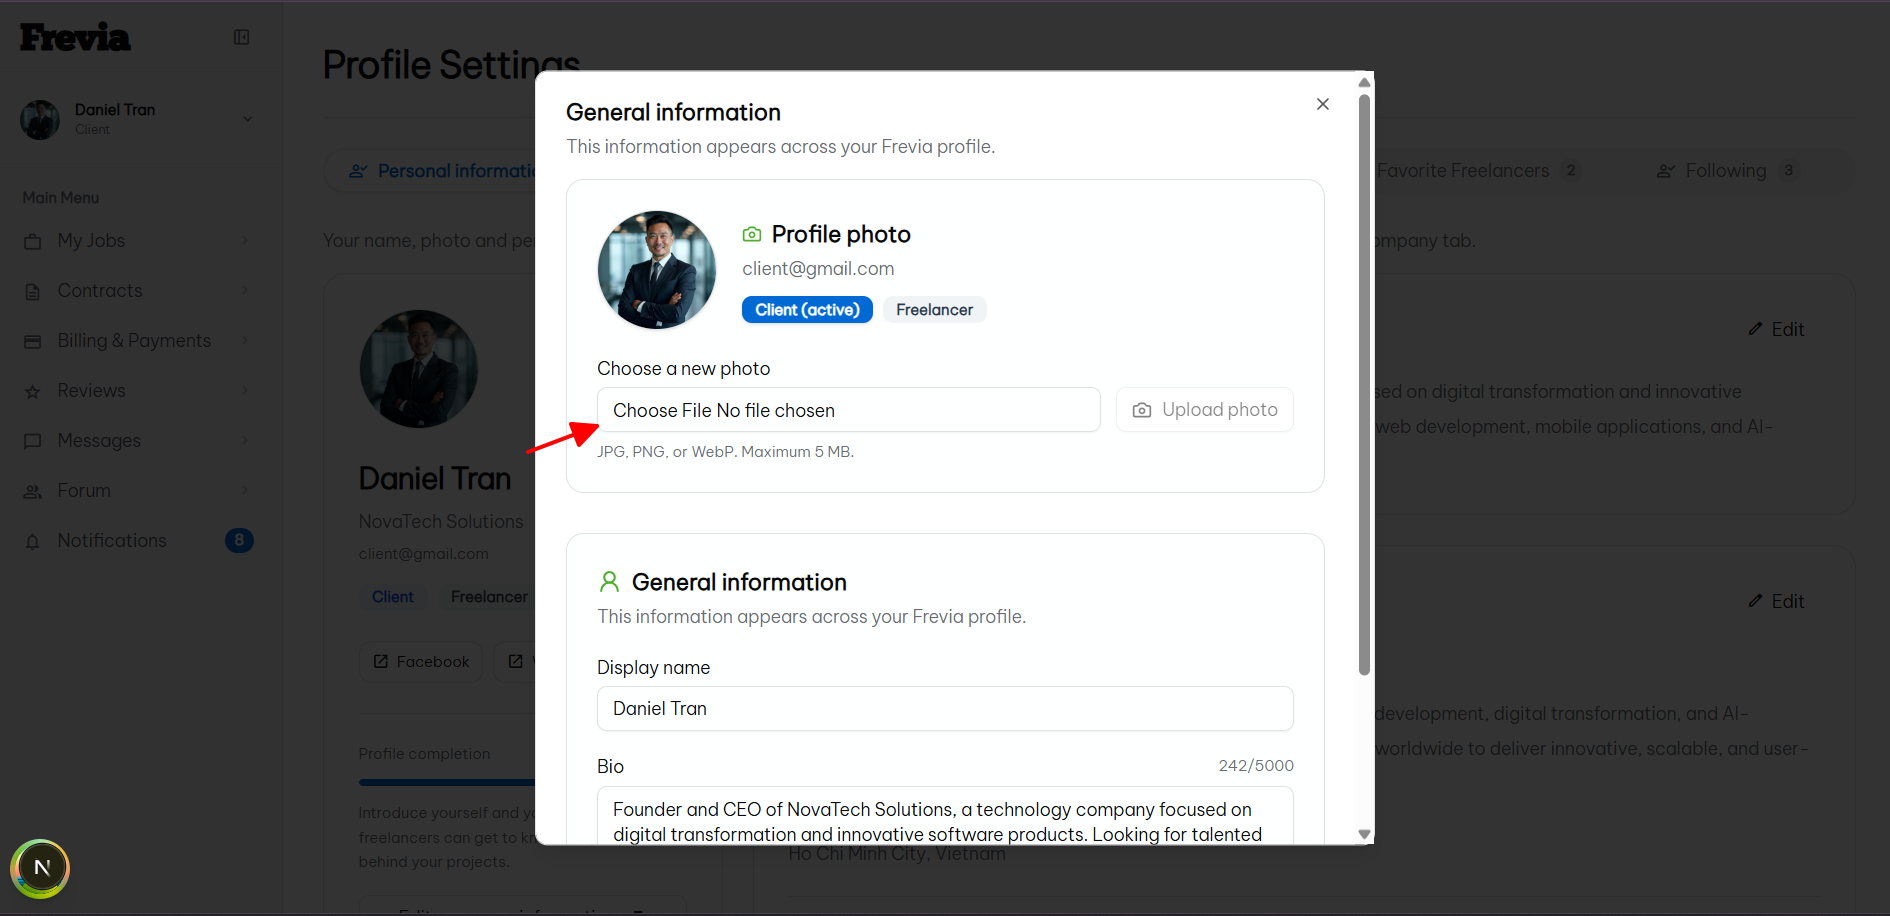
\includegraphics[width=450.00pt]{images/client/m3_02_upload_avatar.png}}
\put(141.30,114.28){\color{fptred}\framebox(121.50,12.00){}}
\put(141.30,126.28){\colorbox{white}{\textcolor{fptred}{\scriptsize\bfseries 1}}}
\put(265.05,114.28){\color{fptred}\framebox(44.10,12.00){}}
\put(265.05,126.28){\colorbox{white}{\textcolor{fptred}{\scriptsize\bfseries 2}}}
\end{picture}
\endgroup}%

\caption{Profile photo selection and upload controls.}
\label{fig:r6_m3_02_upload_avatar}
\end{figure}
\paragraph{Step-by-Step User Instructions:}
\begin{enumerate}[leftmargin=1.8em,itemsep=3pt]
  \item \rbadge{1} Open the photo editor in Personal information. Select Choose a new photo / Choose File.
  \item \rbadge{2} Choose a JPG, PNG or WebP image no larger than 5 MB.
  \item \rbadge{3} Select Upload photo and wait for completion. Confirm the updated avatar before leaving.
\end{enumerate}
\paragraph{Expected Output \& Exception Handling:}
\begin{itemize}[leftmargin=1.5em,itemsep=2pt]
  \item \textbf{Expected result:} The saved avatar appears in the account profile.
  \item \textbf{Troubleshooting:} For an unsupported or oversized file, choose another image. If uploading fails, check connectivity and retry without repeatedly submitting.
\end{itemize}

\newpage
\subsubsection{M3.03 -- Change Password}
\begin{itemize}[leftmargin=1.5em,itemsep=2pt]
  \item \textbf{Screen Name \& Route Path:}\newline \texttt{/freelancer/profile or /client/profile}.
  \item \textbf{Target Actor:} Freelancer or Client.
  \item \textbf{Preconditions:} Signed in with a password-based account.
  \item \textbf{Purpose:} Replace the existing account password.
\end{itemize}
\paragraph{Screen-Transition Workflow:} Personal information $\rightarrow$ bottom of page $\rightarrow$ Change password $\rightarrow$ validation result.
\begin{figure}[H]\centering
\scalebox{0.44931}{%
\begingroup\setlength{\unitlength}{1pt}\linethickness{0.9pt}
\begin{picture}(450.00,217.03)
\put(0,0){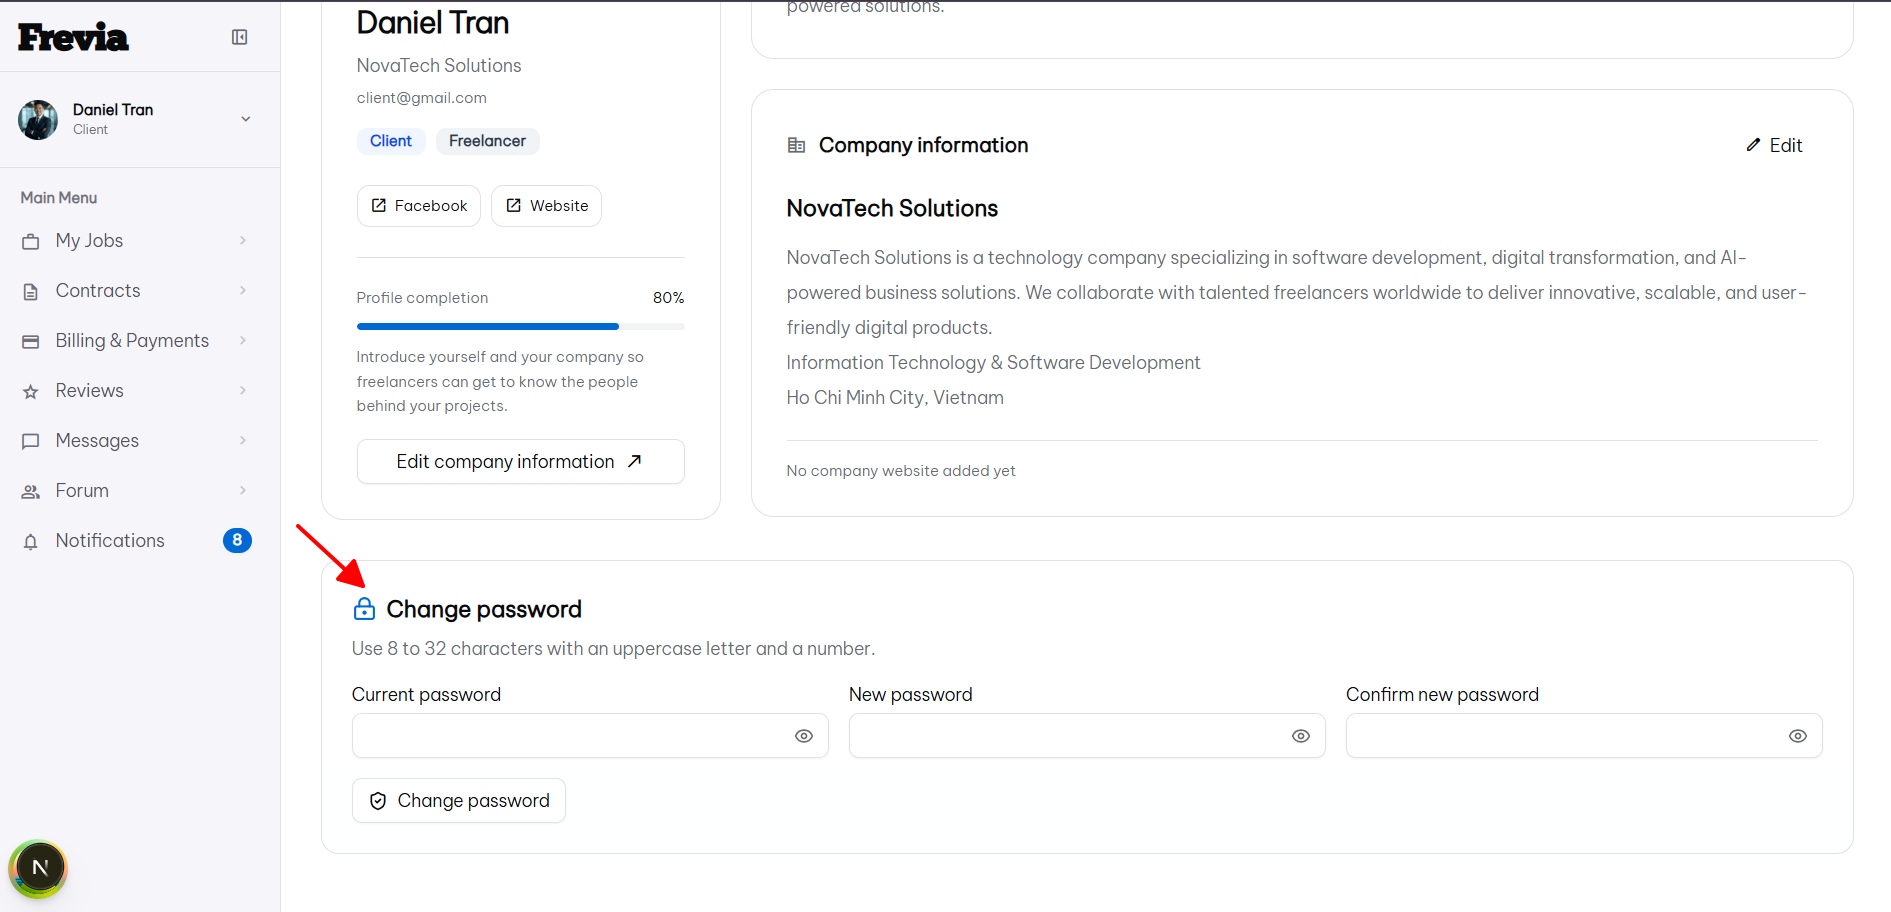
\includegraphics[width=450.00pt]{images/client/m3_03_change_password.png}}
\put(82.80,35.81){\color{fptred}\framebox(351.45,11.94){}}
\put(82.80,47.75){\colorbox{white}{\textcolor{fptred}{\scriptsize\bfseries 1}}}
\put(83.25,20.40){\color{fptred}\framebox(51.75,11.94){}}
\put(83.25,32.34){\colorbox{white}{\textcolor{fptred}{\scriptsize\bfseries 2}}}
\end{picture}
\endgroup}%

\caption{Change password fields and submit action.}
\label{fig:r6_m3_03_change_password}
\end{figure}
\paragraph{Step-by-Step User Instructions:}
\begin{enumerate}[leftmargin=1.8em,itemsep=3pt]
  \item \rbadge{1} Scroll to Change password at the bottom of Personal information.
  \item \rbadge{2} Enter Current password, New password and Confirm new password. Use 8--32 characters, including an uppercase letter and a number.
  \item \rbadge{3} Use the eye icon if needed to verify the entry, then select Change password.
\end{enumerate}
\paragraph{Expected Output \& Exception Handling:}
\begin{itemize}[leftmargin=1.5em,itemsep=2pt]
  \item \textbf{Expected result:} A success notification confirms the password change.
  \item \textbf{Troubleshooting:} If the current password is incorrect, correct it or use the account recovery workflow. If confirmation does not match, re-enter it before submitting.
\end{itemize}

\newpage
\subsubsection{M3.04 -- Manage Social Links}
\begin{itemize}[leftmargin=1.5em,itemsep=2pt]
  \item \textbf{Screen Name \& Route Path:}\newline \texttt{/freelancer/profile?tab=social or /client/profile?tab=social}.
  \item \textbf{Target Actor:} Freelancer or Client.
  \item \textbf{Preconditions:} Signed in; a valid public URL is available.
  \item \textbf{Purpose:} Add, inspect or remove social links.
\end{itemize}
\paragraph{Screen-Transition Workflow:} Profile settings $\rightarrow$ Social links $\rightarrow$ Add link or delete confirmation $\rightarrow$ refreshed list.
\begin{figure}[H]\centering
\scalebox{0.9556}{%
\begingroup\setlength{\unitlength}{1pt}\linethickness{0.9pt}
\begin{picture}(450.00,127.47)
\put(0,0){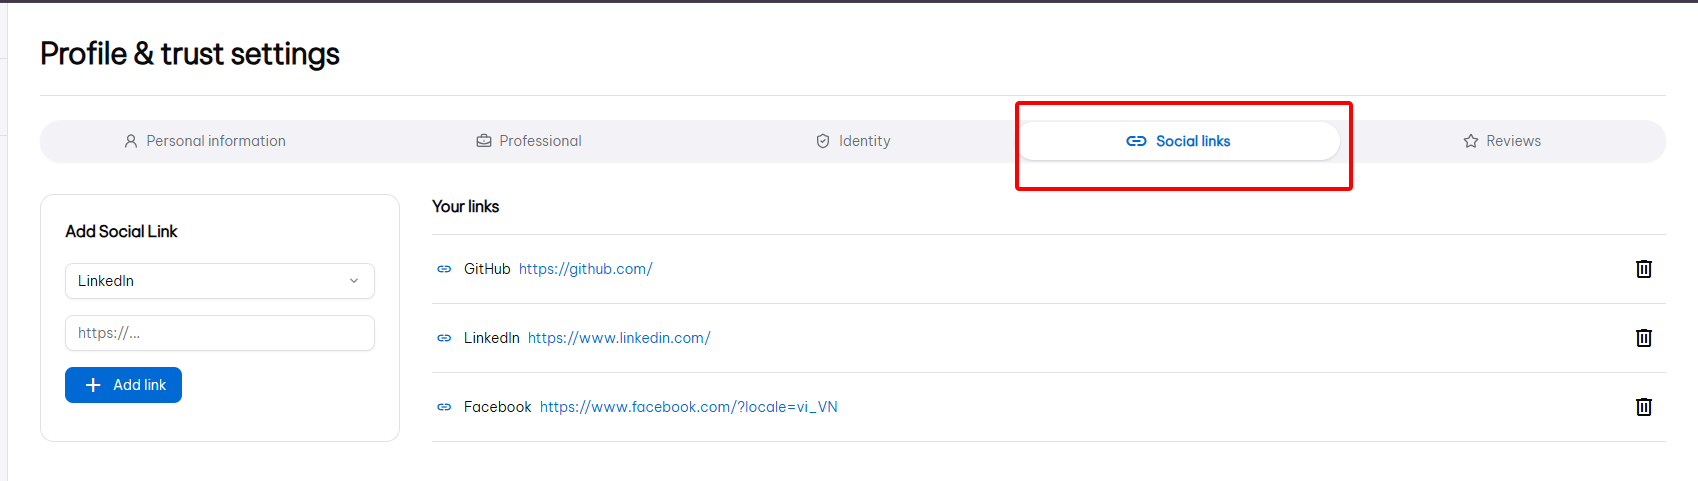
\includegraphics[width=450.00pt]{images/client/m3_04_view_social_link_list.png}}
\put(10.80,10.58){\color{fptred}\framebox(94.50,65.65){}}
\put(10.80,76.23){\colorbox{white}{\textcolor{fptred}{\scriptsize\bfseries 1}}}
\put(114.30,15.17){\color{fptred}\framebox(325.80,59.91){}}
\put(114.30,75.08){\colorbox{white}{\textcolor{fptred}{\scriptsize\bfseries 2}}}
\end{picture}
\endgroup}%

\caption{Social links: platform/URL form and saved links.}
\label{fig:r6_m3_04_view_social_link_list}
\end{figure}
\paragraph{Step-by-Step User Instructions:}
\begin{enumerate}[leftmargin=1.8em,itemsep=3pt]
  \item \rbadge{1} Select Social links and review Your links.
  \item \rbadge{2} To add a link, choose a platform, enter its complete URL and select Add link.
  \item \rbadge{3} To remove a link, select its trash action. Confirm the deletion in the dialog, or select Cancel to keep the link.
  \item \rbadge{4} To replace a URL when no edit action is offered, remove the old entry and add the corrected one.
\end{enumerate}
\paragraph{Expected Output \& Exception Handling:}
\begin{itemize}[leftmargin=1.5em,itemsep=2pt]
  \item \textbf{Expected result:} The list reflects successful additions and removals; cancelling leaves the entry intact.
  \item \textbf{Troubleshooting:} Use a valid URL and avoid adding the same platform twice. On a failed request, keep the current entry and retry after correcting the error.
\end{itemize}

\newpage
\subsubsection{M3.05 -- Join a Marketplace Role}
\begin{itemize}[leftmargin=1.5em,itemsep=2pt]
  \item \textbf{Screen Name \& Route Path:}\newline \texttt{Account menu}.
  \item \textbf{Target Actor:} Client or Freelancer.
  \item \textbf{Preconditions:} Signed in; the other marketplace role has not been joined.
  \item \textbf{Purpose:} Add the other marketplace role to the same account.
\end{itemize}
\paragraph{Screen-Transition Workflow:} Account menu $\rightarrow$ Add Client role or Add Freelancer role $\rightarrow$ role becomes available.
\begin{figure}[H]\centering
\scalebox{0.21348}{%
\begingroup\setlength{\unitlength}{1pt}\linethickness{0.9pt}
\begin{picture}(450.00,1311.60)
\put(0,0){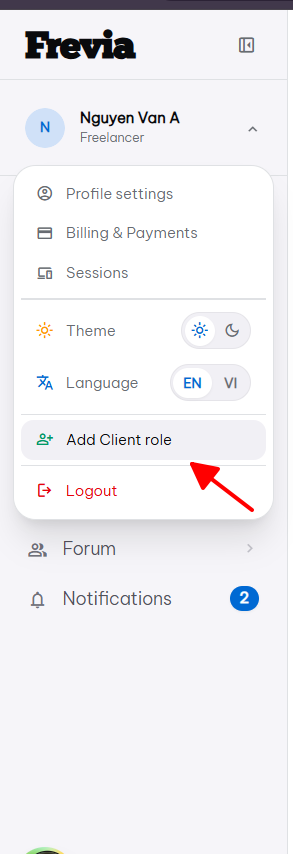
\includegraphics[width=450.00pt]{images/client/m3_05_join_new_role.png}}
\put(32.40,603.34){\color{fptred}\framebox(376.20,62.96){}}
\put(32.40,666.29){\colorbox{white}{\textcolor{fptred}{\scriptsize\bfseries 1}}}
\end{picture}
\endgroup}%

\caption{Account menu: add the other marketplace role.}
\label{fig:r6_m3_05_join_new_role}
\end{figure}
\paragraph{Step-by-Step User Instructions:}
\begin{enumerate}[leftmargin=1.8em,itemsep=3pt]
  \item \rbadge{1} Open the account menu.
  \item \rbadge{2} Choose Add Client role when using a Freelancer account, or the corresponding Add Freelancer role action for a Client account.
  \item \rbadge{3} Wait for confirmation and inspect the available role-switch action.
\end{enumerate}
\paragraph{Expected Output \& Exception Handling:}
\begin{itemize}[leftmargin=1.5em,itemsep=2pt]
  \item \textbf{Expected result:} The account gains the requested marketplace role without creating a second login.
  \item \textbf{Troubleshooting:} An already assigned role is not added again. Expert and Administrator access cannot be self-assigned using this menu.
\end{itemize}

\newpage
\subsubsection{M3.06 -- Switch Active Role}
\begin{itemize}[leftmargin=1.5em,itemsep=2pt]
  \item \textbf{Screen Name \& Route Path:}\newline \texttt{Account menu}.
  \item \textbf{Target Actor:} Client and Freelancer role holder.
  \item \textbf{Preconditions:} The account already has both marketplace roles.
  \item \textbf{Purpose:} Change the active workspace.
\end{itemize}
\paragraph{Screen-Transition Workflow:} Account menu $\rightarrow$ Switch to Client/Freelancer $\rightarrow$ corresponding workspace.
\begin{figure}[H]\centering
\scalebox{0.22174}{%
\begingroup\setlength{\unitlength}{1pt}\linethickness{0.9pt}
\begin{picture}(450.00,1262.76)
\put(0,0){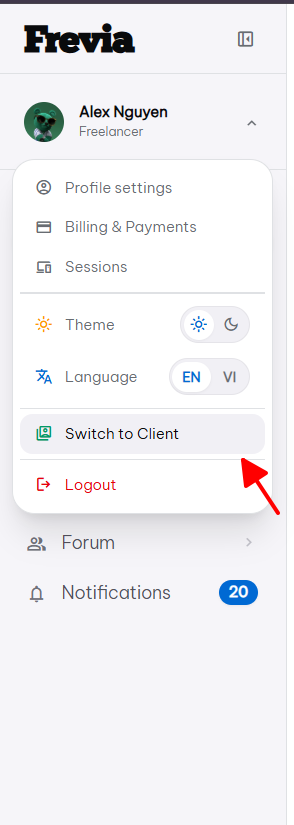
\includegraphics[width=450.00pt]{images/client/m3_06_switch_role.png}}
\put(30.60,566.98){\color{fptred}\framebox(374.85,60.61){}}
\put(30.60,627.59){\colorbox{white}{\textcolor{fptred}{\scriptsize\bfseries 1}}}
\end{picture}
\endgroup}%

\caption{Account menu: switch the active marketplace role.}
\label{fig:r6_m3_06_switch_role}
\end{figure}
\paragraph{Step-by-Step User Instructions:}
\begin{enumerate}[leftmargin=1.8em,itemsep=3pt]
  \item \rbadge{1} Open the account menu.
  \item \rbadge{2} Select Switch to Client or Switch to Freelancer, as appropriate.
  \item \rbadge{3} Wait for navigation, then verify the active role and sidebar before performing an operation.
\end{enumerate}
\paragraph{Expected Output \& Exception Handling:}
\begin{itemize}[leftmargin=1.5em,itemsep=2pt]
  \item \textbf{Expected result:} The workspace and available actions match the selected active role.
  \item \textbf{Troubleshooting:} If the target role is absent, join it first using M3.05. A permission error after switching should be retried after refreshing the session.
\end{itemize}

\newpage
\subsubsection{M7.01 -- Open Client Workspace}
\begin{itemize}[leftmargin=1.5em,itemsep=2pt]
  \item \textbf{Screen Name \& Route Path:}\newline \texttt{/dashboard (redirects to /client/jobs)}.
  \item \textbf{Target Actor:} Client.
  \item \textbf{Preconditions:} Signed in with Client as the active role.
  \item \textbf{Purpose:} Reach the Client job-management workspace.
\end{itemize}
\paragraph{Screen-Transition Workflow:} Sign in or switch to Client $\rightarrow$ Dashboard $\rightarrow$ My Jobs.
\begin{figure}[H]\centering
\scalebox{0.65778}{%
\begingroup\setlength{\unitlength}{1pt}\linethickness{0.9pt}
\begin{picture}(450.00,281.25)
\put(0,0){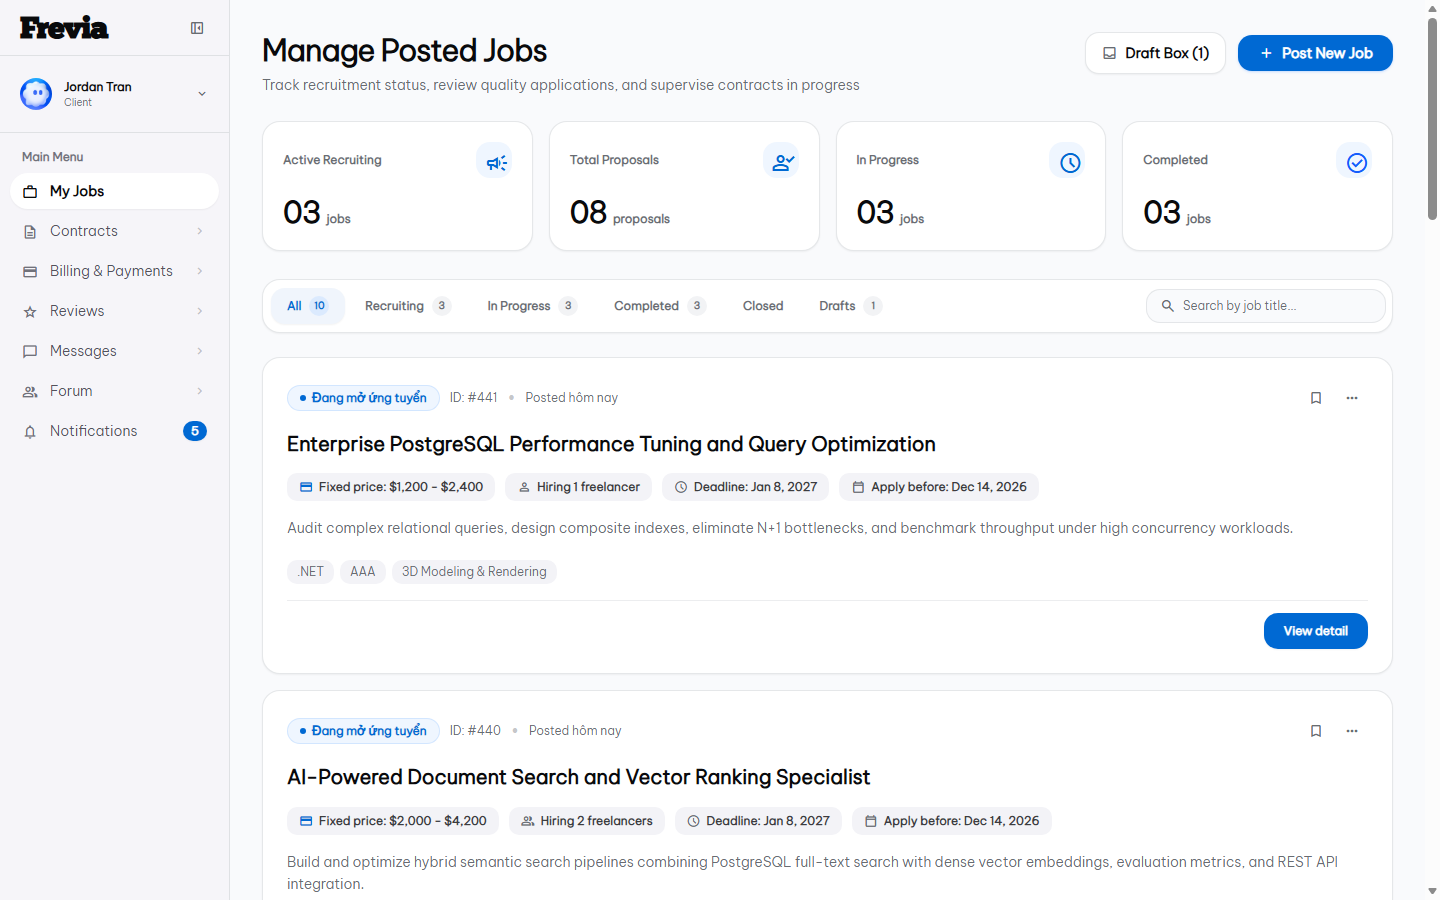
\includegraphics[width=450.00pt]{images/client/m7_01_client_workspace.png}}
\put(3.15,215.16){\color{fptred}\framebox(65.25,12.38){}}
\put(3.15,227.53){\colorbox{white}{\textcolor{fptred}{\scriptsize\bfseries 1}}}
\put(81.45,202.22){\color{fptred}\framebox(354.15,41.91){}}
\put(81.45,244.12){\colorbox{white}{\textcolor{fptred}{\scriptsize\bfseries 2}}}
\put(81.90,177.47){\color{fptred}\framebox(353.25,16.31){}}
\put(81.90,193.78){\colorbox{white}{\textcolor{fptred}{\scriptsize\bfseries 3}}}
\end{picture}
\endgroup}%
\caption{Client workspace at My Jobs; example data varies by account.}
\label{fig:r6_m7_01_client_workspace}
\end{figure}
\paragraph{Step-by-Step User Instructions:}
\begin{enumerate}[leftmargin=1.8em,itemsep=3pt]
  \item \rbadge{1} Activate the Client role.
  \item \rbadge{2} Open \texttt{/dashboard}; the current application forwards Client accounts to \texttt{/client/jobs}.
  \item \rbadge{3} Use the Client navigation for jobs, proposals, contracts and profile settings.
\end{enumerate}
\paragraph{Expected Output \& Exception Handling:}
\begin{itemize}[leftmargin=1.5em,itemsep=2pt]
  \item \textbf{Expected result:} The Client reaches the authorized workspace.
  \item \textbf{Troubleshooting:} If directed to another workspace, inspect the active role. Summary cards and job counts depend on the signed-in Client; use the status tabs and search field to locate jobs.
\end{itemize}

\newpage
\subsubsection{M7.02 -- Update Company Information}
\begin{itemize}[leftmargin=1.5em,itemsep=2pt]
  \item \textbf{Screen Name \& Route Path:}\newline \texttt{/client/profile?tab=company}.
  \item \textbf{Target Actor:} Client.
  \item \textbf{Preconditions:} Signed in; Client is the active role.
  \item \textbf{Purpose:} Maintain published company information.
\end{itemize}
\paragraph{Screen-Transition Workflow:} Personal information $\rightarrow$ Edit company information $\rightarrow$ Company profile $\rightarrow$ save or review.
\begin{figure}[H]\centering
\scalebox{0.9476}{%
\begingroup\setlength{\unitlength}{1pt}\linethickness{0.9pt}
\begin{picture}(450.00,221.62)
\put(0,0){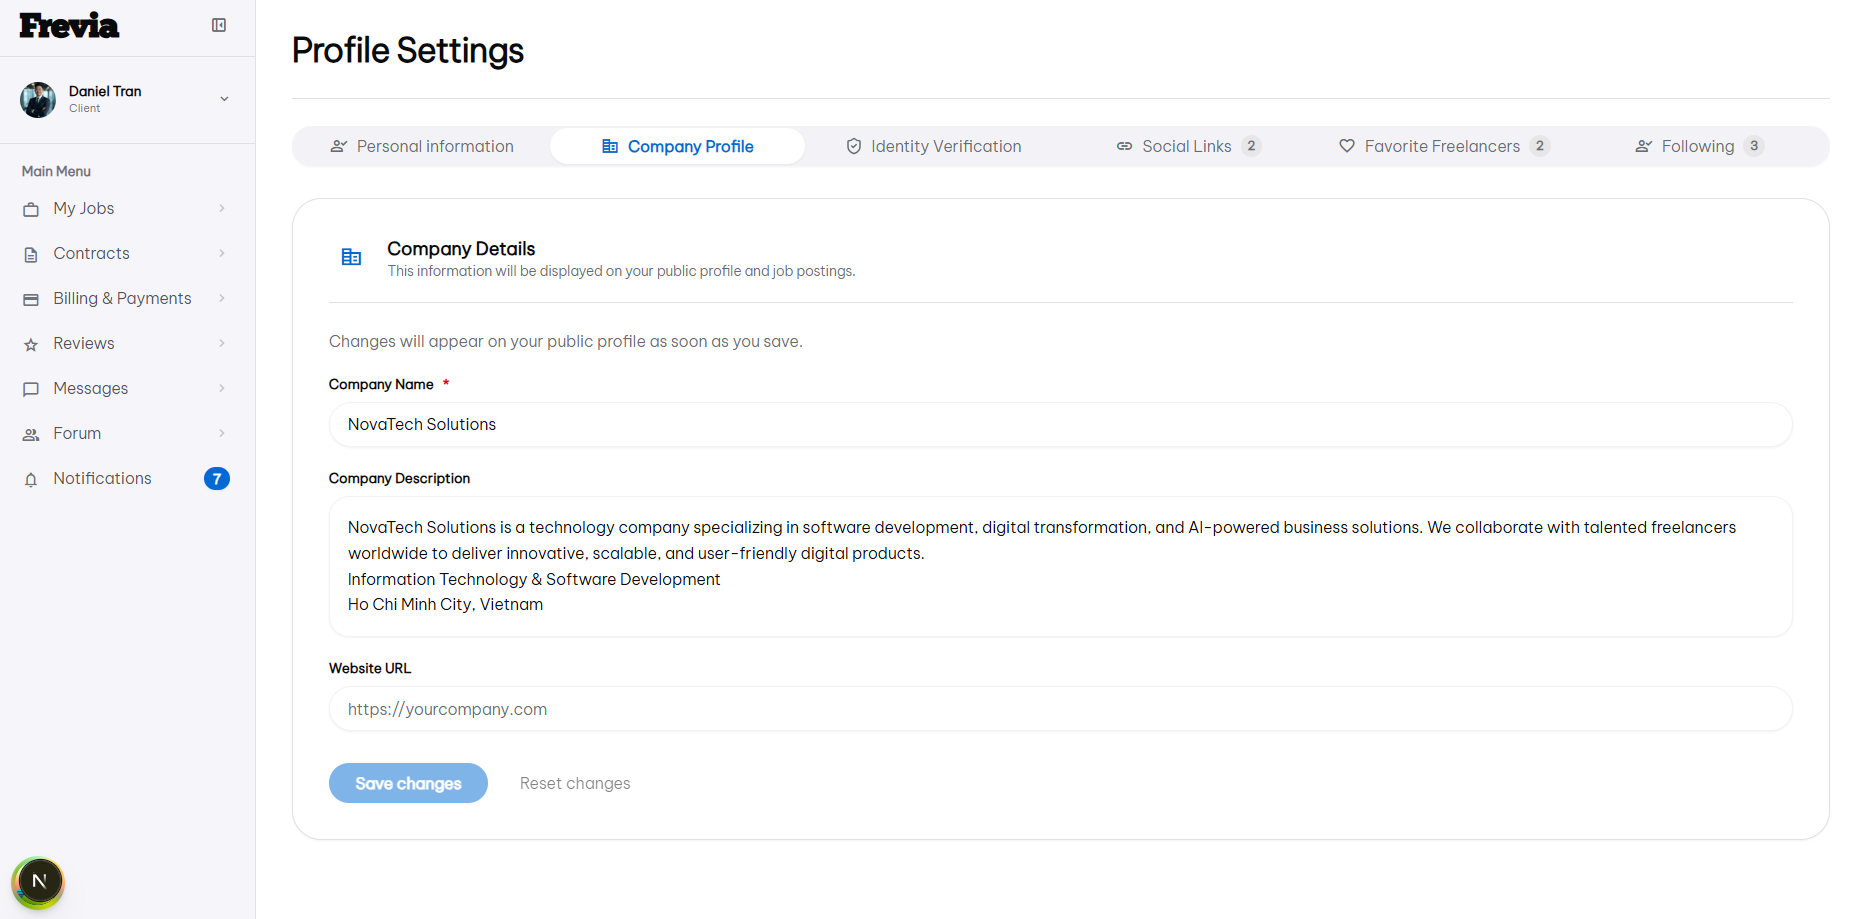
\includegraphics[width=450.00pt]{images/client/m7_02_update_company_information.png}}
\put(78.30,44.32){\color{fptred}\framebox(353.70,82.00){}}
\put(78.30,126.32){\colorbox{white}{\textcolor{fptred}{\scriptsize\bfseries 1}}}
\put(78.30,27.70){\color{fptred}\framebox(39.60,11.30){}}
\put(78.30,39.01){\colorbox{white}{\textcolor{fptred}{\scriptsize\bfseries 2}}}
\end{picture}
\endgroup}%

\caption{Company profile editor and save action.}
\label{fig:r6_m7_02_update_company_information}
\end{figure}
\paragraph{Step-by-Step User Instructions:}
\begin{enumerate}[leftmargin=1.8em,itemsep=3pt]
  \item \rbadge{1} Select Company profile, or use Edit company information from the Personal information overview.
  \item \rbadge{2} Update Company name, Company description and Website. Use a valid website URL when provided.
  \item \rbadge{3} Save the company form and inspect the resulting message. Return to Personal information to view the published company summary.
\end{enumerate}
\paragraph{Expected Output \& Exception Handling:}
\begin{itemize}[leftmargin=1.5em,itemsep=2pt]
  \item \textbf{Expected result:} Approved company details appear in the overview; a pending revision remains a draft until approved.
  \item \textbf{Troubleshooting:} Do not repeatedly save a pending proposal to force publication. Correct validation errors or follow the rejection notes.
\end{itemize}

\newpage
\subsubsection{M7.03 -- Manage Favorite Freelancers}
\begin{itemize}[leftmargin=1.5em,itemsep=2pt]
  \item \textbf{Screen Name \& Route Path:}\newline \texttt{/client/profile?tab=favorites}.
  \item \textbf{Target Actor:} Client.
  \item \textbf{Preconditions:} Signed in as Client; target is another Freelancer.
  \item \textbf{Purpose:} Save and remove a personal shortlist.
\end{itemize}
\paragraph{Screen-Transition Workflow:} Freelancer profile $\rightarrow$ favorite action $\rightarrow$ Favorite freelancers tab $\rightarrow$ remove or view profile.
\begin{figure}[H]\centering
\begin{minipage}[c]{0.48\textwidth}\centering
\scalebox{0.47775}{%
\begingroup\setlength{\unitlength}{1pt}\linethickness{0.9pt}
\begin{picture}(450.00,252.09)
\put(0,0){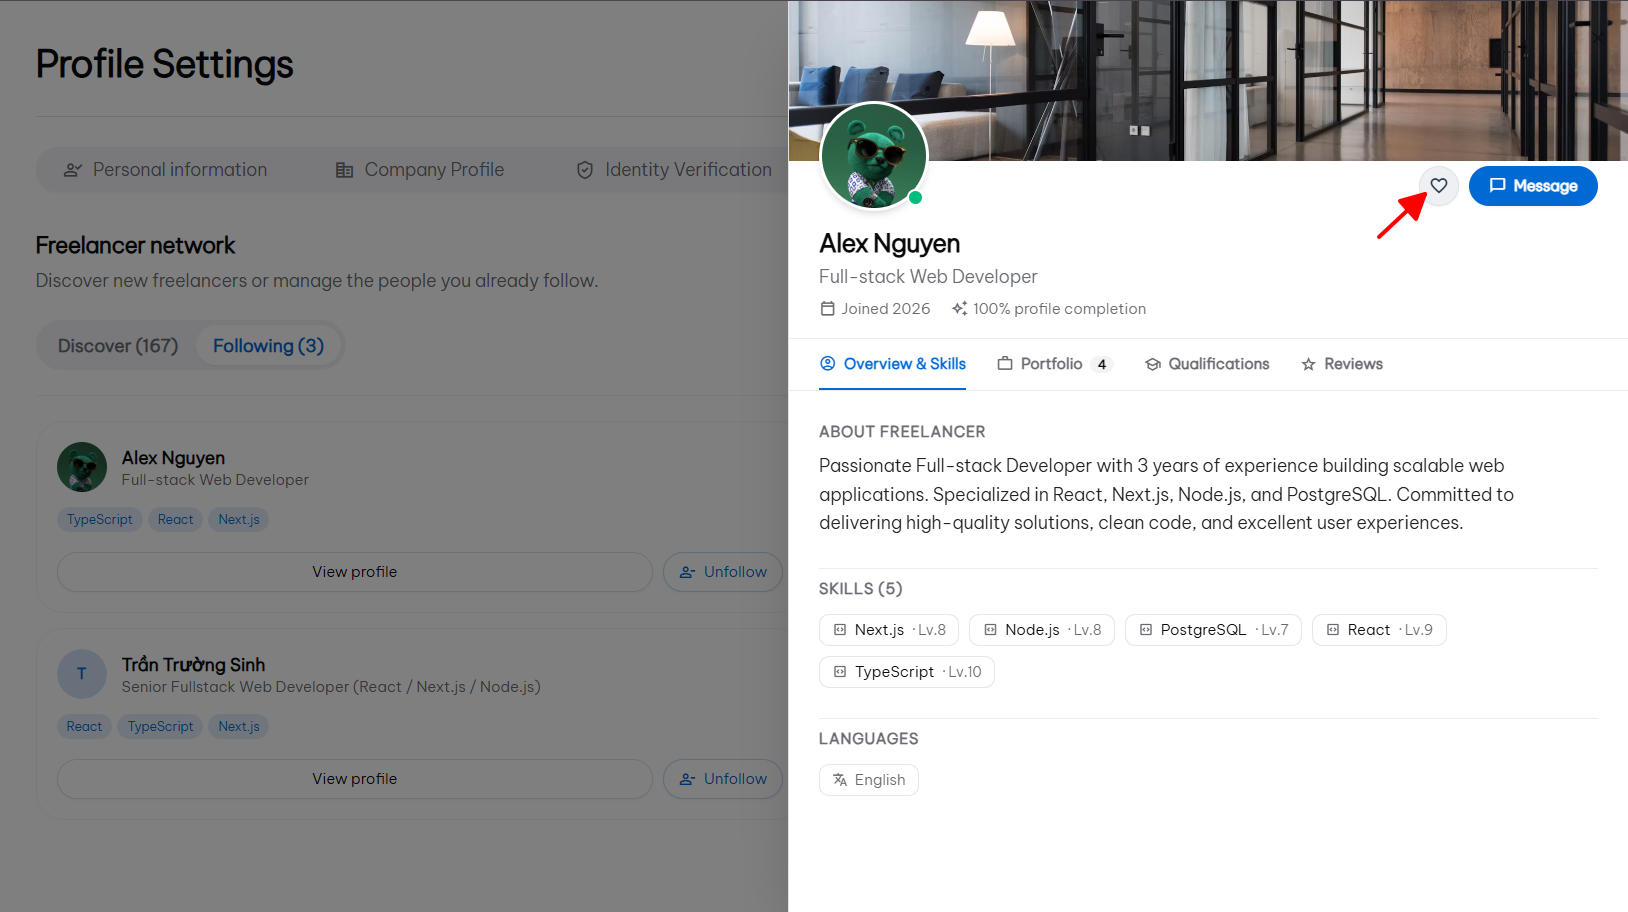
\includegraphics[width=450.00pt]{images/client/m7_03_add_freelancer_to_favorites.png}}
\put(391.05,193.35){\color{fptred}\framebox(13.05,13.11){}}
\put(391.05,206.46){\colorbox{white}{\textcolor{fptred}{\scriptsize\bfseries 1}}}
\end{picture}
\endgroup}%
\end{minipage}\hfill
\begin{minipage}[c]{0.48\textwidth}\centering
\scalebox{0.29697}{%
\begingroup\setlength{\unitlength}{1pt}\linethickness{0.9pt}
\begin{picture}(450.00,251.44)
\put(0,0){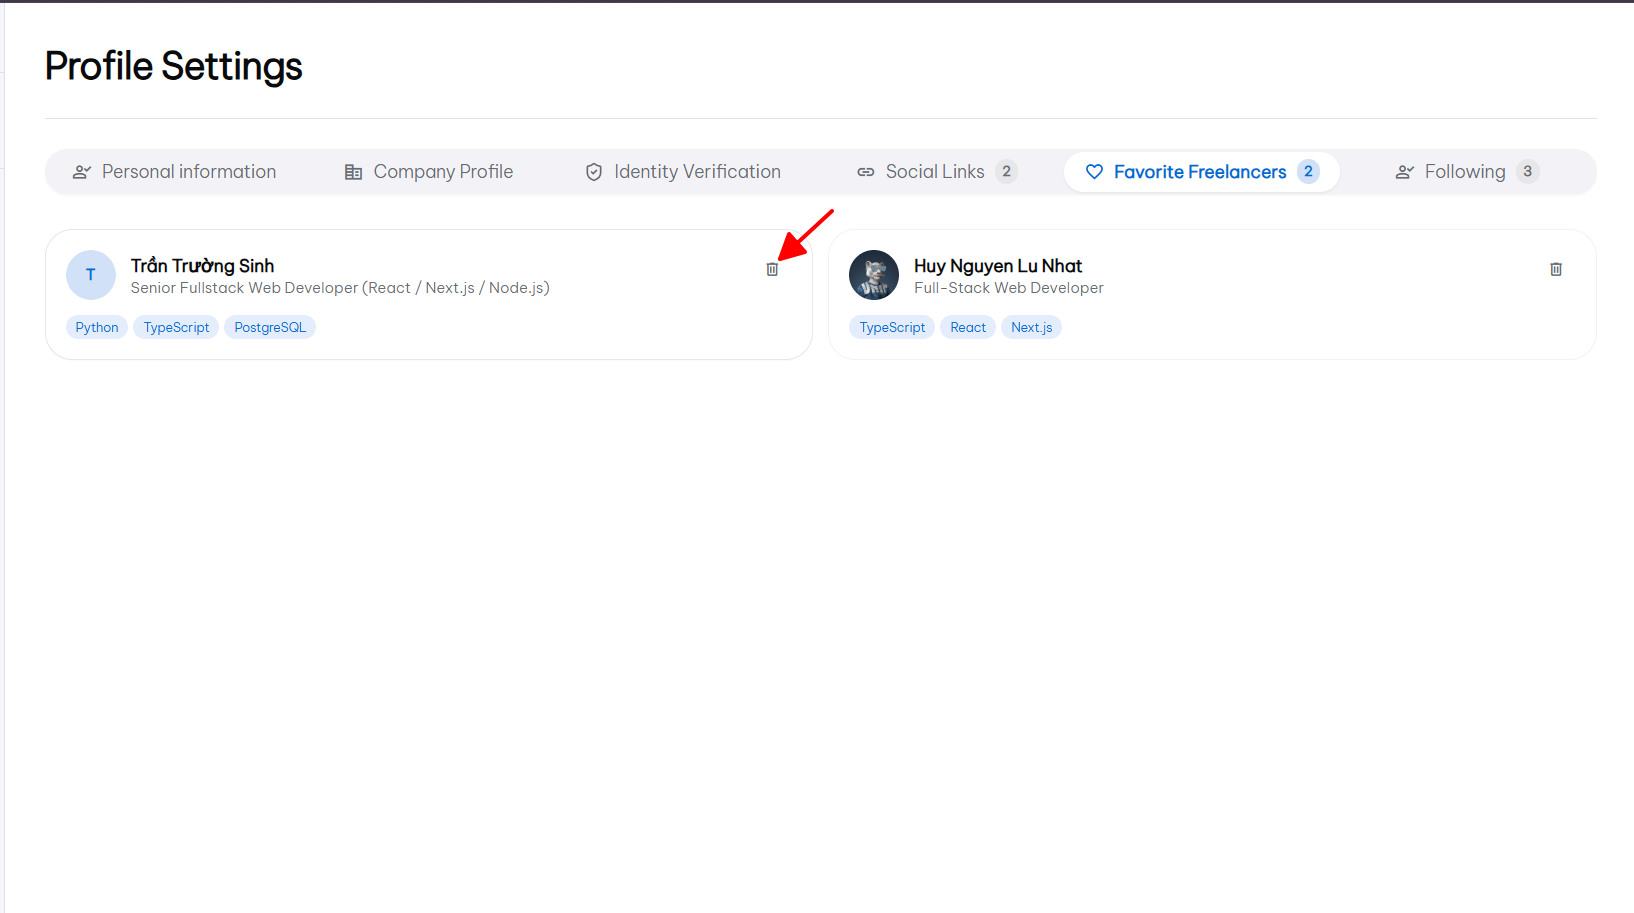
\includegraphics[width=450.00pt]{images/client/m7_03_remove_freelancer_from_favorites.png}}
\put(207.90,169.72){\color{fptred}\framebox(12.15,13.07){}}
\put(207.90,182.80){\colorbox{white}{\textcolor{fptred}{\scriptsize\bfseries 1}}}
\end{picture}
\endgroup}%
\end{minipage}
\caption{Add a Freelancer to favorites from the public profile (left); favorite freelancers tab and remove action.}
\label{fig:r6_m7_03_add_freelancer_to_favorites}
\label{fig:r6_m7_03_remove_freelancer_from_favorites}
\end{figure}
\paragraph{Step-by-Step User Instructions:}
\begin{enumerate}[leftmargin=1.8em,itemsep=3pt]
  \item \rbadge{1} Open the Freelancer public profile. Select Favorite; the profile preview may display a heart action beside Message.
  \item \rbadge{2} Open Client profile settings and select Favorite freelancers to see the shortlist.
  \item \rbadge{3} Select a listed profile to inspect it. Use its remove action to remove the favorite; verify that it disappears after success.
\end{enumerate}
\paragraph{Expected Output \& Exception Handling:}
\begin{itemize}[leftmargin=1.5em,itemsep=2pt]
  \item \textbf{Expected result:} Adding fills the favorite state and places the Freelancer in the Client shortlist; removing clears both.
  \item \textbf{Troubleshooting:} Use the Client role and another user's Freelancer profile. If a request fails, retry after connectivity is restored; do not assume the favorite was saved.
\end{itemize}

\newpage
\subsubsection{M7.04 -- Manage Following List}
\begin{itemize}[leftmargin=1.5em,itemsep=2pt]
  \item \textbf{Screen Name \& Route Path:}\newline \texttt{/client/profile?tab=following}.
  \item \textbf{Target Actor:} Client.
  \item \textbf{Preconditions:} Signed in; a Freelancer is available to follow.
  \item \textbf{Purpose:} Discover and follow Freelancers.
\end{itemize}
\paragraph{Screen-Transition Workflow:} Profile settings $\rightarrow$ Following $\rightarrow$ Discover or Following list $\rightarrow$ Follow/Unfollow.
\begin{figure}[H]\centering
\begin{minipage}[c]{0.48\textwidth}\centering
\scalebox{0.43506}{%
\begingroup\setlength{\unitlength}{1pt}\linethickness{0.9pt}
\begin{picture}(450.00,256.66)
\put(0,0){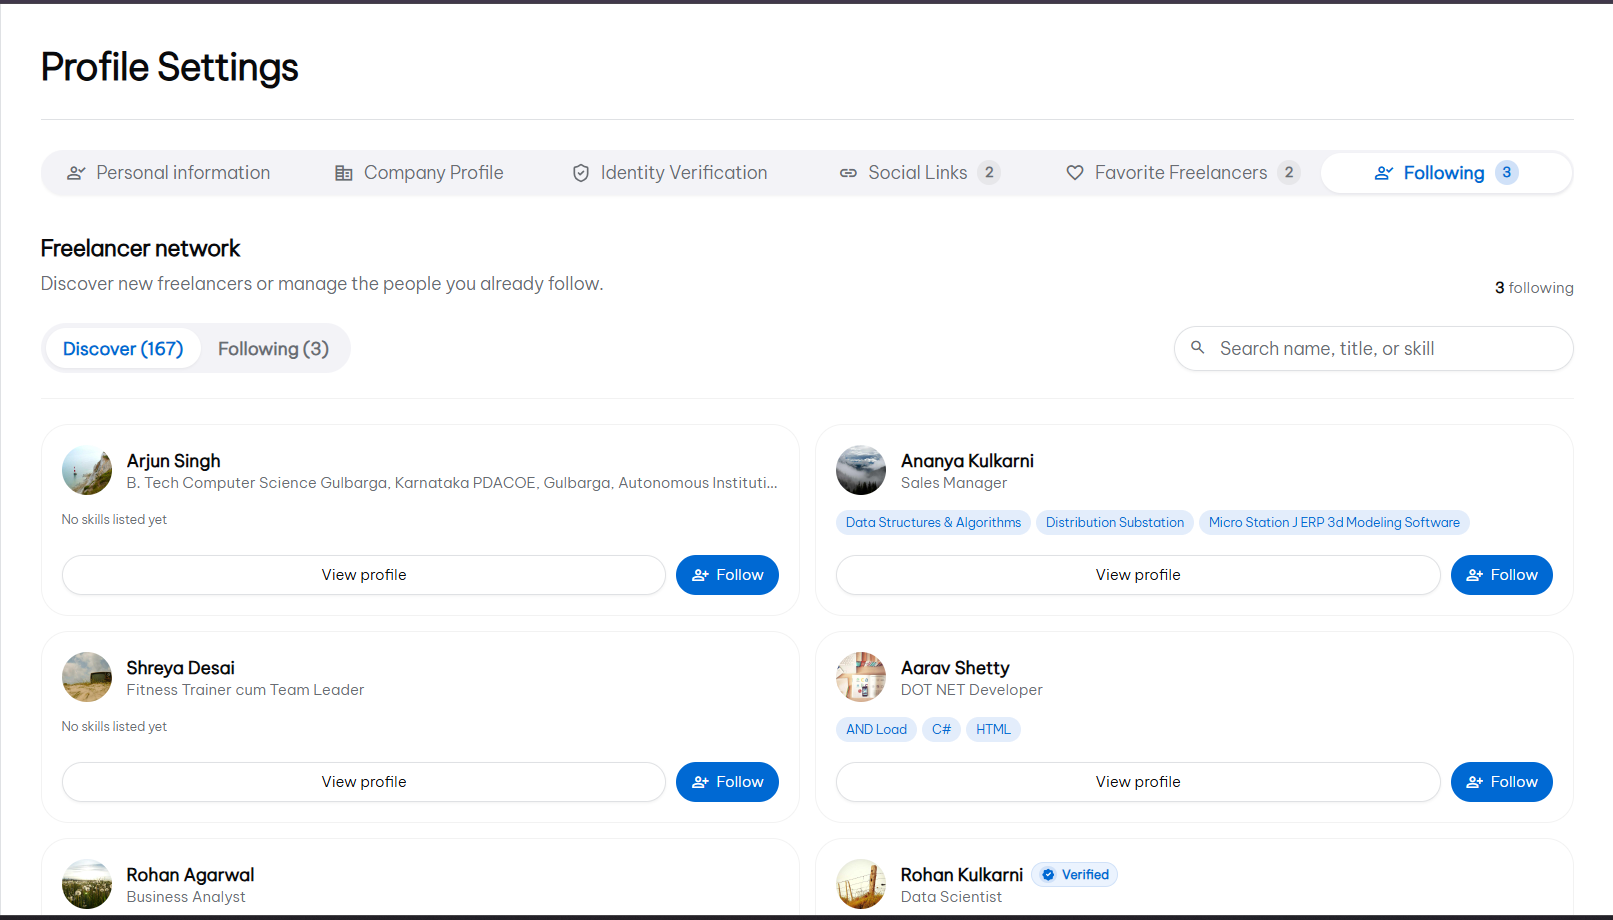
\includegraphics[width=450.00pt]{images/client/m7_04_view_following_list.png}}
\put(11.70,151.17){\color{fptred}\framebox(87.30,14.37){}}
\put(11.70,165.55){\colorbox{white}{\textcolor{fptred}{\scriptsize\bfseries 1}}}
\put(187.65,89.06){\color{fptred}\framebox(30.15,12.58){}}
\put(187.65,101.64){\colorbox{white}{\textcolor{fptred}{\scriptsize\bfseries 2}}}
\end{picture}
\endgroup}%
\end{minipage}\hfill
\begin{minipage}[c]{0.48\textwidth}\centering
\scalebox{0.33775}{%
\begingroup\setlength{\unitlength}{1pt}\linethickness{0.9pt}
\begin{picture}(450.00,229.42)
\put(0,0){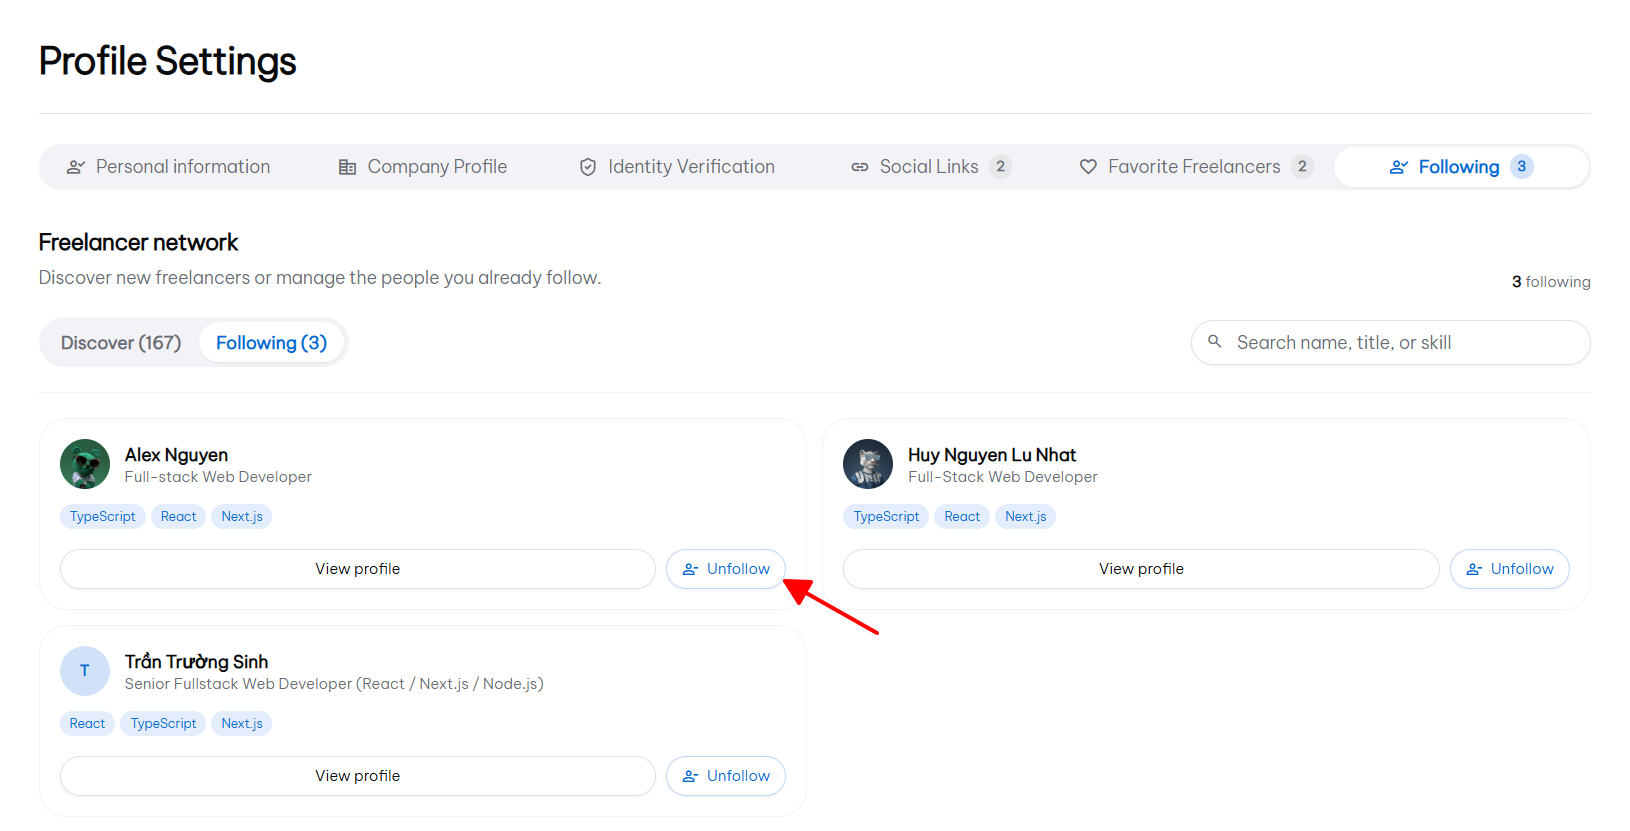
\includegraphics[width=450.00pt]{images/client/m7_04_unfollow_freelancer.png}}
\put(183.60,66.99){\color{fptred}\framebox(36.00,13.31){}}
\put(183.60,80.30){\colorbox{white}{\textcolor{fptred}{\scriptsize\bfseries 1}}}
\end{picture}
\endgroup}%
\end{minipage}
\caption{Following workspace: Discover and Following lists (left); unfollow action on a followed Freelancer card.}
\label{fig:r6_m7_04_view_following_list}
\label{fig:r6_m7_04_unfollow_freelancer}
\end{figure}
\paragraph{Step-by-Step User Instructions:}
\begin{enumerate}[leftmargin=1.8em,itemsep=3pt]
  \item \rbadge{1} Select Following in Client profile settings.
  \item \rbadge{2} Use Discover and the name/title/skill search to find a Freelancer. Select Follow on the target card.
  \item \rbadge{3} Switch to the Following list to inspect followed Freelancers. Select View profile or Unfollow as needed.
\end{enumerate}
\paragraph{Expected Output \& Exception Handling:}
\begin{itemize}[leftmargin=1.5em,itemsep=2pt]
  \item \textbf{Expected result:} The following list and count update after successful requests.
  \item \textbf{Troubleshooting:} Following and favorites are separate lists. Removing one relationship does not imply removing the other. Retry a failed load instead of interpreting it as an empty list.
\end{itemize}
